\documentclass{standalone}

\usepackage{tikz}
\usetikzlibrary{decorations.pathreplacing,calligraphy}

\begin{document}
	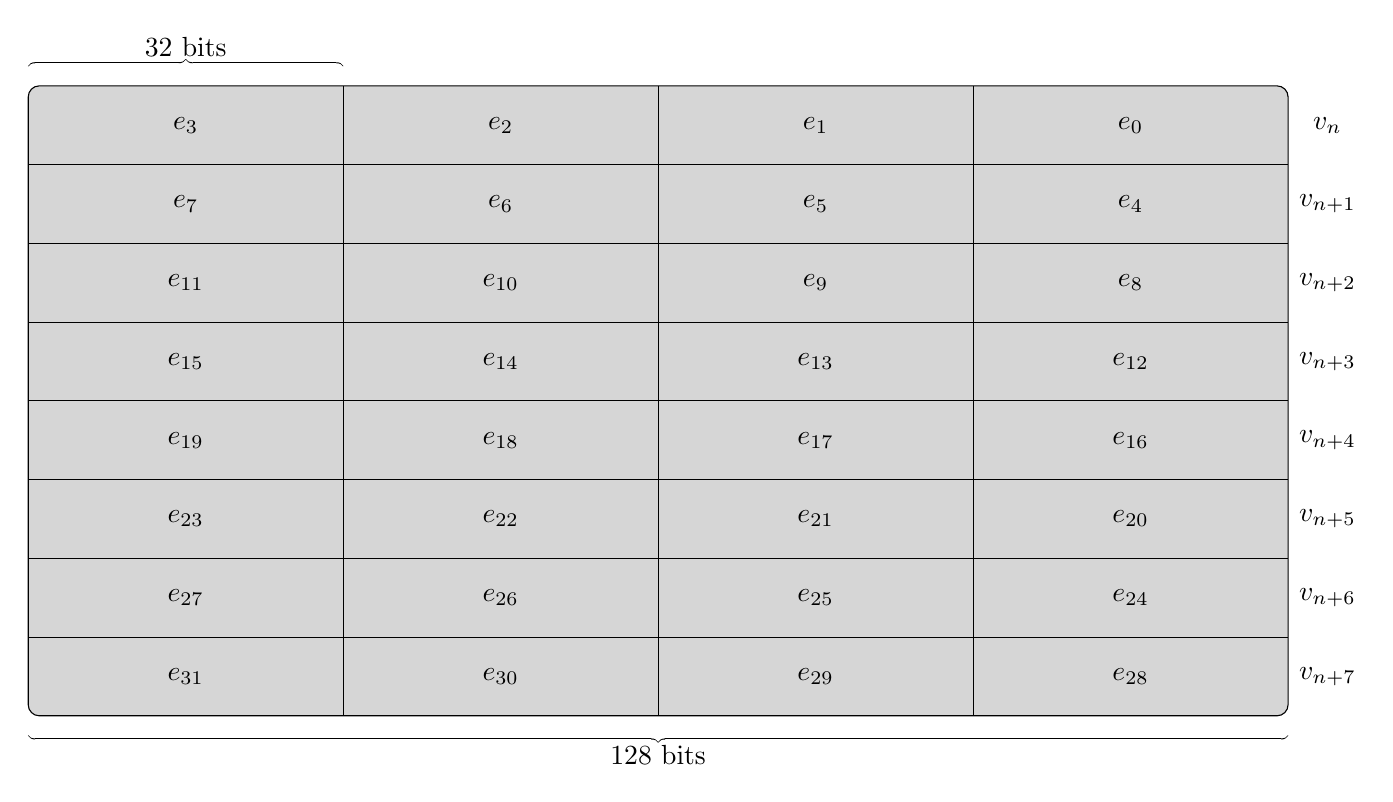
\begin{tikzpicture}
		\draw[fill=gray!32, rounded corners] (0, 0) rectangle (16, 8);
		\draw (4, 0) -- (4, 8);
		\draw (8, 0) -- (8, 8);
		\draw (12, 0) -- (12, 8);
		\draw (0, 1) -- (16, 1);
		\draw (0, 2) -- (16, 2);
		\draw (0, 3) -- (16, 3);
		\draw (0, 4) -- (16, 4);
		\draw (0, 5) -- (16, 5);
		\draw (0, 6) -- (16, 6);
		\draw (0, 7) -- (16, 7);
		
		\node at (2, 7.5) {$e_{3}$};
		\node at (6, 7.5) {$e_{2}$};
		\node at (10, 7.5) {$e_{1}$};
		\node at (14, 7.5) {$e_{0}$};
		
		\node at (2, 6.5) {$e_{7}$};
		\node at (6, 6.5) {$e_{6}$};
		\node at (10, 6.5) {$e_{5}$};
		\node at (14, 6.5) {$e_{4}$};
		
		\node at (2, 5.5) {$e_{11}$};
		\node at (6, 5.5) {$e_{10}$};
		\node at (10, 5.5) {$e_{9}$};
		\node at (14, 5.5) {$e_{8}$};
		
		\node at (2, 4.5) {$e_{15}$};
		\node at (6, 4.5) {$e_{14}$};
		\node at (10, 4.5) {$e_{13}$};
		\node at (14, 4.5) {$e_{12}$};
		
		\node at (2, 3.5) {$e_{19}$};
		\node at (6, 3.5) {$e_{18}$};
		\node at (10, 3.5) {$e_{17}$};
		\node at (14, 3.5) {$e_{16}$};
		
		\node at (2, 2.5) {$e_{23}$};
		\node at (6, 2.5) {$e_{22}$};
		\node at (10, 2.5) {$e_{21}$};
		\node at (14, 2.5) {$e_{20}$};
		
		\node at (2, 1.5) {$e_{27}$};
		\node at (6, 1.5) {$e_{26}$};
		\node at (10, 1.5) {$e_{25}$};
		\node at (14, 1.5) {$e_{24}$};
		
		\node at (2, 0.5) {$e_{31}$};
		\node at (6, 0.5) {$e_{30}$};
		\node at (10, 0.5) {$e_{29}$};
		\node at (14, 0.5) {$e_{28}$};
		
		\draw [decorate, decoration = {calligraphic brace}] (0, 8.25) --  (4, 8.25);
		\draw [decorate, decoration = {calligraphic brace, mirror}] (0, -0.25) --  (16, -0.25); 
		
		\node at (2, 8.5) {32 bits};
		\node at (8, -0.5) {128 bits};
		
		\node at (16.5, 7.5) {$v_{n}$};
		\node at (16.5, 6.5) {$v_{n+1}$};
		\node at (16.5, 5.5) {$v_{n+2}$};
		\node at (16.5, 4.5) {$v_{n+3}$};
		\node at (16.5, 3.5) {$v_{n+4}$};
		\node at (16.5, 2.5) {$v_{n+5}$};
		\node at (16.5, 1.5) {$v_{n+6}$};
		\node at (16.5, 0.5) {$v_{n+7}$};
	\end{tikzpicture}
\end{document}t